\section{Afgrænsning}
Til at afgrænse projektet anvendes \textbf{M}o\textbf{SC}o\textbf{W} modellen, som beskriver hvilke dele projektet skal (\textbf{M}ust), bør (\textbf{S}houd), kan (\textbf{C}ould og ikke (\textbf{W}ont) indeholde. MoSCoW modellen (figur: \ref{fig:moscow}) viser hvordan de enkelte krav og dele af projektet er prioriteret. 
Redegørelse og begrundelser for valg/fravalg
Moscow

\begin{figure}[H]
	\centering
	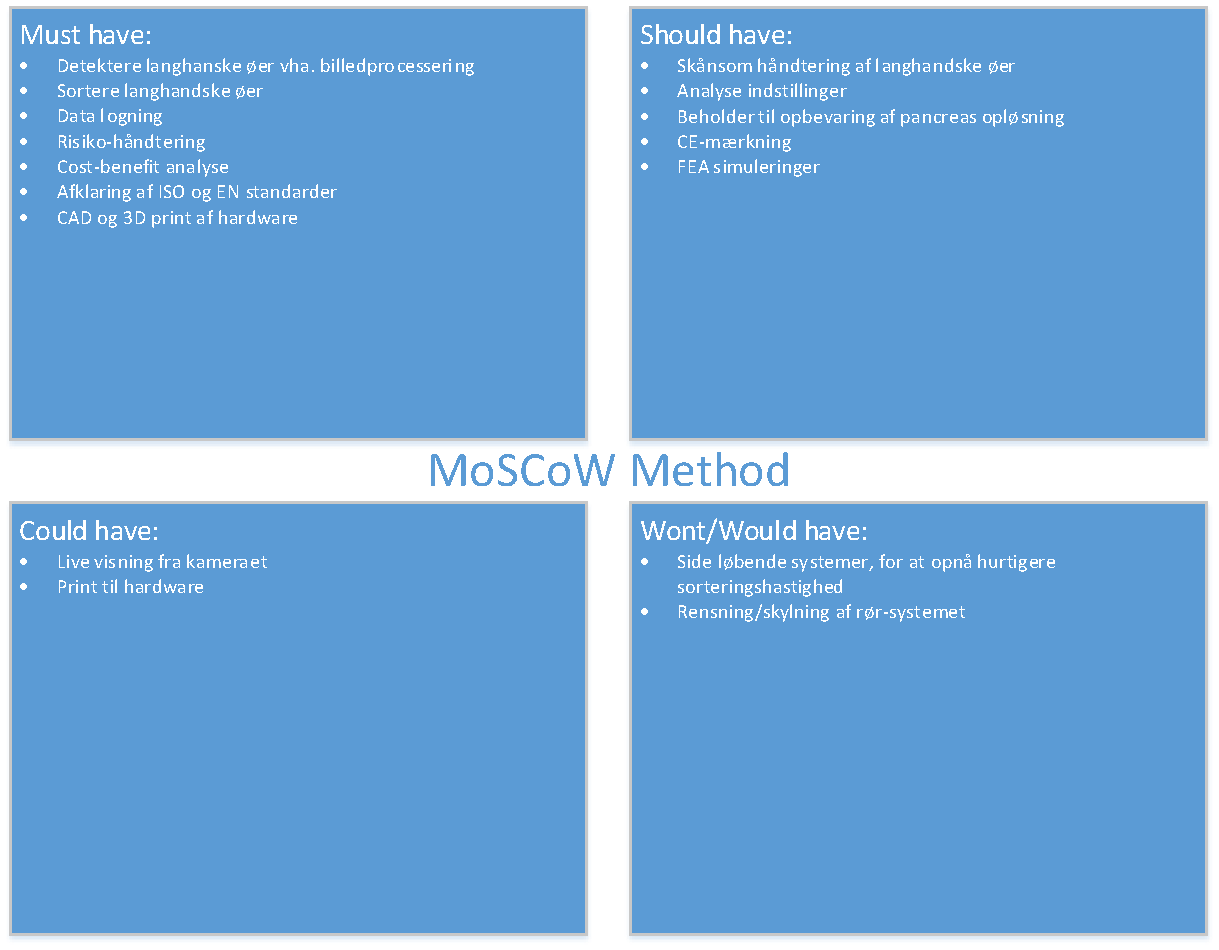
\includegraphics[width=1\textwidth]{billeder/MoSCoW-crop.pdf}
	\caption{MoSCoW}
	\label{fig:moscow}
\end{figure}

De krav systemet skal opfylde er bl.a. at kunne detektere langerhanske øer vha. billedprocessering, samt sortere øerne ved detektion. Herudover skal systemet kunne gemme data omkring de sorterede øer herunder størrelse og cirkularitet. Projektet består desuden af en cost-benefit analyse der beskriver hvilke fordele og ulemper det automatiserede system vil have. 

Et af de vigtigere krav der er nedprioteriet i projektet er skånsom håndtering af langerhanske øer. Denne del vil kræve en validering af den udviklede prototype igennem funktionstest af de isolerede langerhanske øer. Referencer til dette?

Dette projekt vil derfor i højere grad fokusere på en verificering af den udviklede prototype i form af en accepttest, som tester de funktionelle og ikke funktionelle krav.
